\documentclass[a4paper]{article}
\usepackage{amsfonts}
\usepackage{amsmath}
\usepackage{amssymb}
\usepackage{graphicx}
\newcommand{\dint}{\displaystyle\int}     

\begin{document}
  
\noindent \large Auteur: Etienne El Hachem \\
\noindent \large Studierichting: Informatica\\
\noindent \large Oefeningenreeks 5D nr. 3.4\\

\medskip

\normalsize

$f(x) = \sec^2x$ en $g(x) = \sec x \cdot \tan x$\\

$\dint\limits_{-\tfrac{\pi}{3}}^{\tfrac{\pi}{6}} (\sec^2x - \sec x \cdot \tan x)dx$\\

$= \dint\limits_{-\tfrac{\pi}{3}}^{\tfrac{\pi}{6}} \left(\dfrac{1}{\cos^2x} - \dfrac{\sin x}{\cos^2x}\right)dx$\\

$= \dint\limits_{-\tfrac{\pi}{3}}^{\tfrac{\pi}{6}} \dfrac{1}{\cos^2x} dx - \dint\limits_{-\tfrac{\pi}{3}}^{\tfrac{\pi}{6}} \dfrac{\sin x}{\cos^2x}dx$\\

$= \left[\tan x\right]_{-\tfrac{\pi}{3}}^{\tfrac{\pi}{6}} - \left[\sec x\right]_{-\tfrac{\pi}{3}}^{\tfrac{\pi}{6}}$\\

$= \dfrac{\sqrt{3}}{3} + \sqrt{3} - \dfrac{2\sqrt{3}}{3} + 2 = \dfrac{2\sqrt{3}}{3} + 2$\\

\begin{figure}[h]
\centering
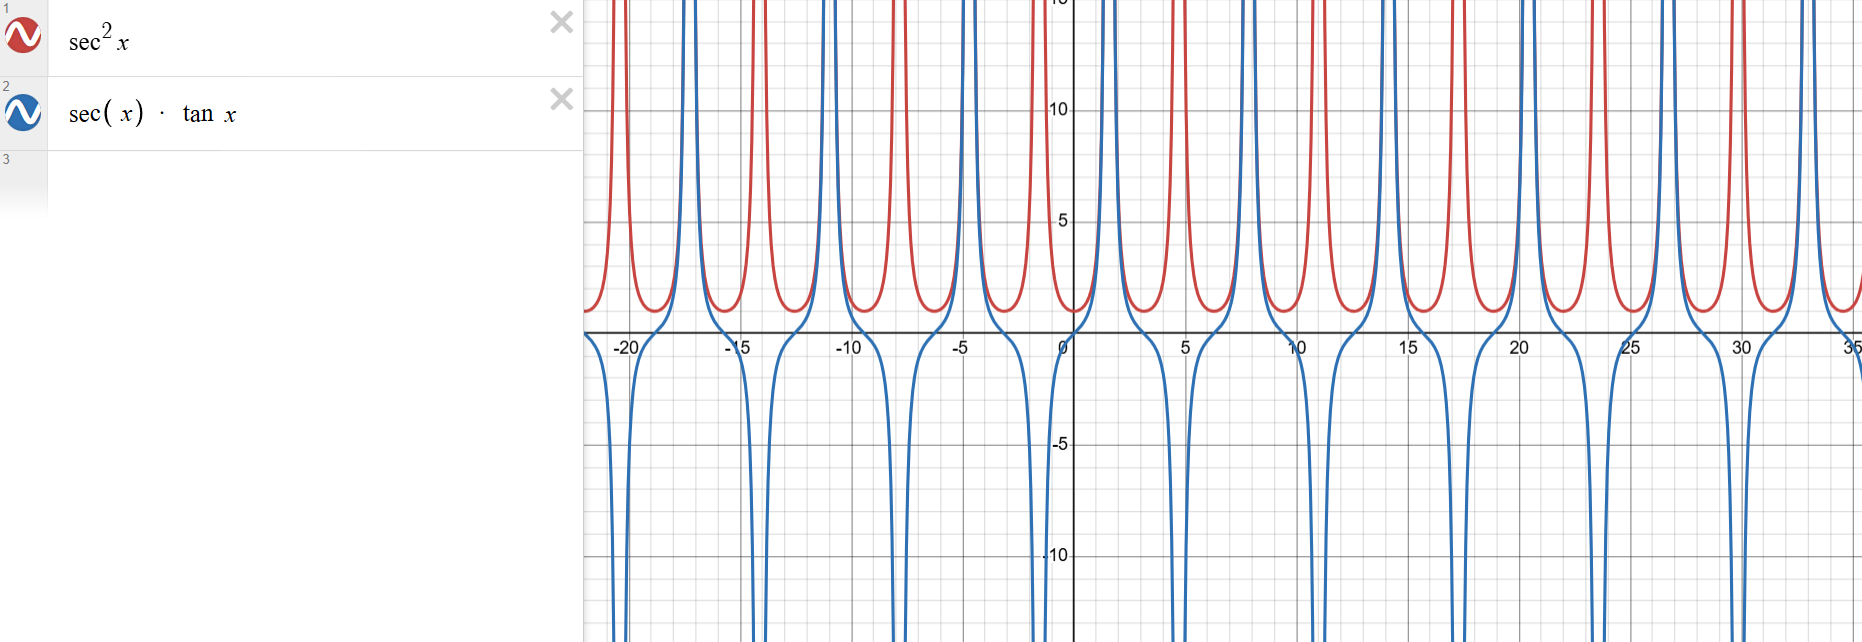
\includegraphics[width=10cm]{5D-3.4-etienne.el.hachem.INF.png}
\end{figure}

\begin{thebibliography}{999}
%\bibitem{a} Referentie
\end{thebibliography}
\end{document} 
